\chapter{Proceso}

Para la realización de este proyecto, se utilizará el proceso de software 'Prototipo'; proceso que permite generar iteraciones en las que se genera un prototipo en cada una, que será expuesto a pruebas y labores de mantenimiento para iniciar la siguiente iteración. Todo esto con la finalidad de obtener un producto final que cumpla con todos los requerimientos plantados para el buen funcionamiento.

\begin{figure}[h!]
	\centering
	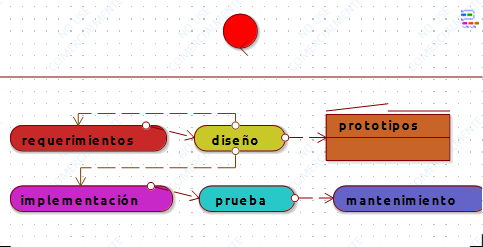
\includegraphics[width=0.7\linewidth]{proyecto/proceso/imgs/prototipo}
	\caption{Proceso Prototipo}
\end{figure}
\section{Implementación}

El proyecto será estructurado como un conjunto de módulos o componentes, los cuales serán organizados en una escala de dependencia, siendo desarrollados del más independiente al más dependiente. El proceso 'Prototipo' permitirá realizar una iteración por cada módulo propuesto, sin descartar hacer subiteraciones dentro de cada iteración; esto permitirá construir el prototipo final componente por componente. Es de aclarar que un componente no será agregado al prototipo final hasta que no esté totalmente depurado y funcional, proceso que facilitan la iteraciones.


\subsection{Módulos}

*agregar imagen diagrama de componentes*

*descripcion de cada modulo*

*diagrama de gannt*